\chapter{Dinámica del sólido rígido}

\begin{miparrafo}
	Un cuerpo rígido es un caso especial de sistemas de muchas partículas en el cual las distancias entre todas sus componentes permanecen constantes bajo la acción de una fuerza o momento.
	
	Un cuerpo rígido conservará, pues, su forma durante su movimiento. Podemos distinguir dos tipos de movimientos en un sólido rígido:
	
	\begin{itemize}
		\item El movimiento es de \emph{traslación} cuando todas las partículas describen lineas paralelas.
		\item El movimiento es de \emph{rotación} alrededor de un eje cuando todas las partículas describen trayectorias circulares alrededor de una línea llamada \emph{eje de roración}.	
	\end{itemize}
	
	El movimiento más general de un sólido rígido puede considerarse como una combinación de una traslación y una rotación.

\begin{multicols}{2}
$\quad$ 

El movimiento del $CM$ es \textbf{como si} se tratase de una partícula cuya masa sea igual la masa del cuerpo y sobre la que actúa una fuerza igual a la suma de todas las fuerzas exteriores aplicadas al cuerpo.
\begin{figure}[H]
	\centering
	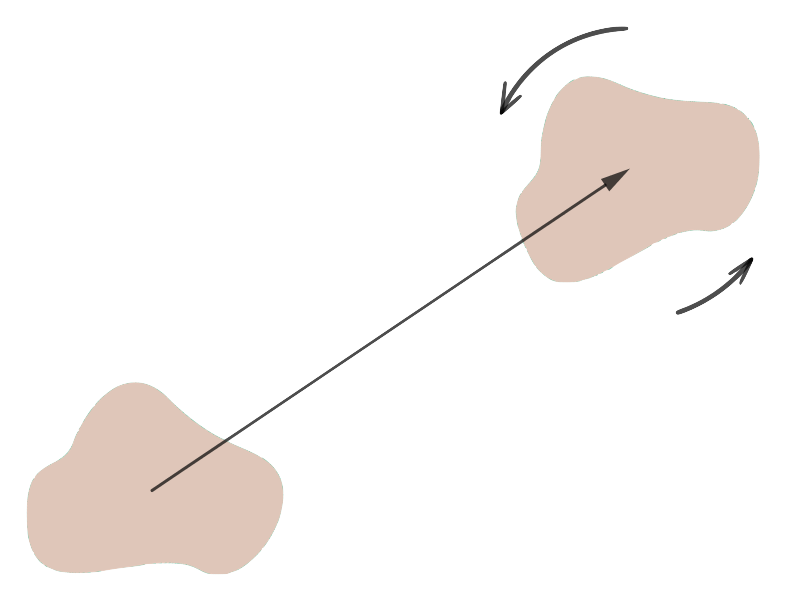
\includegraphics[width=.3\textwidth]{imagenes/imagenes16/T16IM01.png}
\end{figure}
\end{multicols}

$\boldsymbol{ \displaystyle m\dv{\vec v_{CM}}{t}=\vec F^{(e)} }$

En este capítulo nos centraremos en el movimiento de rotación del un cuerpo rígido alrededor de un eje que pase por un punto fijo de un sistema inercia, 
$\displaystyle \boldsymbol{\dv{\vec L}{t}=\vec M^{(e)}}$, o a través de su $CM$, $\ \displaystyle \boldsymbol{\dv{\vec L_{CM}}{t}=\vec M_{CM}^{(e)}}$
\end{miparrafo}

\section{Momento angular de un cuerpo rígido}

\begin{multicols}{2}
Consideremos un cuerpo rígido que gira alrededor de un eje $Z$ con velocidad angular $\vec \omega$.

Cada una de sus partículas describirá una órbita circular centrada en el eje $Z$. Por ejemplo, la partícula $A_i$ describe un círculo de radio $\vec R_i=\overrightarrow{A_iB_1}$, con una velocidad $\vec v_i=\vec \omega \times \vec r_i$, siendo $\vec r_i$ el vector de posición de la partícula $i$ respecto al origen $\mathcal O$, que se escogerá como un punto fijo de un sistema inercial o el centro de masas del cuerpo.
\begin{figure}[H]
	\centering
	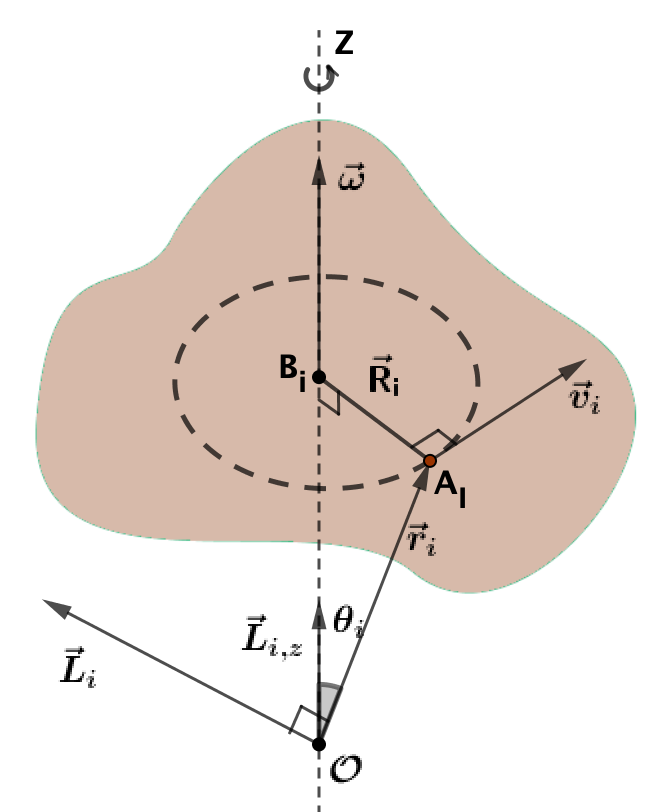
\includegraphics[width=.3\textwidth]{imagenes/imagenes16/T16IM02.png}
\end{figure}
\end{multicols}

En módulo, $\ v_i=\omega r_i \sin \theta_i=\omega R_i$ \textcolor{gris}{$\ \omega$ es la misma para todas las partículas del cuerpo rígido.}

El momento angular de la partícula sita en $A_i$ respecto al origen $\mathcal O$, es:
$\vec L_i=m\vec r_i \times \vec v_i$. Su dirección es $\bot$ al plano formafo por los vectores $\vec r_i \text{ y } \vec v_i$ y está contenido en el plano formado por $\vec r_i$ el eje $Z$, forma un ángulo de $90^o$ con $\vec r_i$ y de $90^o - \theta$ con el eje de rotación $Z$.

La componente de $\vec L_i$ en el eje $Z$ es: $\ L_{iz}=m_ir_iv_i \cos (90^o-\theta_i)$

$L_{iz}=m_ir_iv_i
\sin \theta_i=\textcolor{gris}{(\ v_i=\omega R_i \ )}=mr_i (\omega R_i) \sin \theta_i =m_i R_i^2 \omega$ 

Obsérvese que este resultado es equivalente al de una partícula que se desplaza en un círculo.

La componente en el eje $Z$ del momento angular de todo el cuerpo será:

$L_z=\displaystyle \sum_i L_{iz}=\sum_i m_i R_i^2\ \omega$

\vspace{7mm} %*********************************
Llamamos \emph{\textbf{Momento de Inercia, $I$}} a la expresión:

\vspace{-3mm} %*********************************
\begin{equation} 
\subrayado{\ I=\sum_i m_i R_i^2	\ } \quad \to \qquad  \subrayado{ \ L_z=I\ \omega \ }
\end{equation}


El momento angular de todo el cuerpo es $\ \vec L=\sum_i \vec L_i \ $ en general no es paralelo al eje de rotación.

\vspace{7mm} %*********************************
Para cada cuerpo hay algún eje de rotación para el cual el momento angular total es paralelo al eje. Para cada cuerpo, sin importar su forma, hay tres direcciones perpendiculares para las que el momento angular es paralelo al eje de rotación, estas tres direcciones son los llamados \emph{ejes principales de inercia}, $X_0, Y_0, Z_0$ y a sus momentos de inercia correspondientes les llamaremos \emph{momentos principales de inercia}, que denotaremos por $I_1, I_2, I_3$. Los ejes principales de inercia constituyen un sistema de referencia fijo en el cuerpo que rota respecto al observador.

\begin{figure}[H]
	\centering
	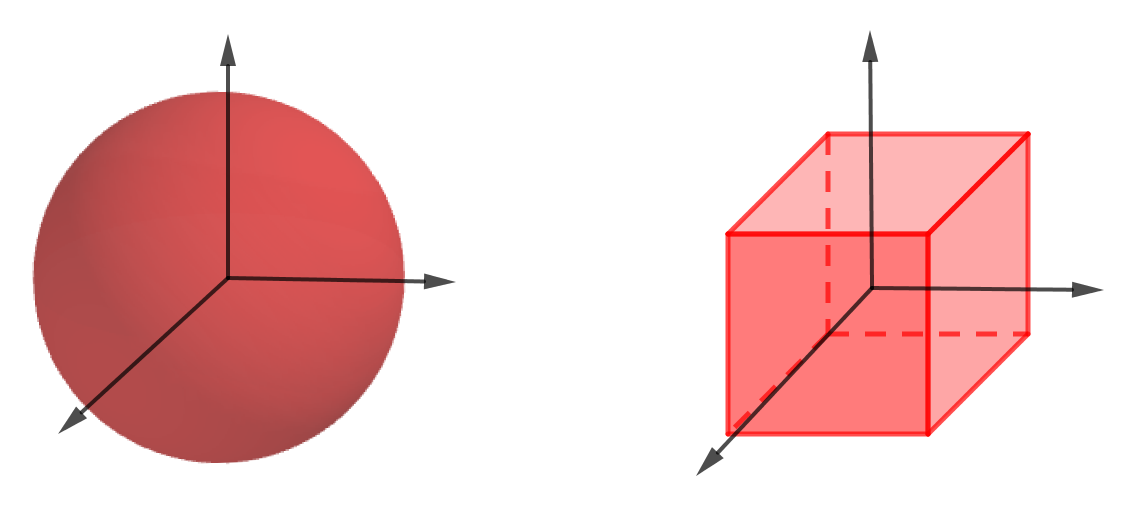
\includegraphics[width=.75\textwidth]{imagenes/imagenes16/T16IM03.png}
\end{figure}


Los ejes principales de inercia en cuerpos simétricos coinciden con ejes de simetría.

Cuando el cuerpo rota alrededor de un eje principal de inercia, $\vec L \ || \ \vec \omega\ $ \textcolor{gris}{($\vec \omega$ siempre en el eje de rotación)}. Podremos escribir, en este caso:

\begin{equation}
\subrayado{\vec L \ = \ I \ \vec \omega}	
\end{equation}

donde $I$ representa el momento principal de inercia correspondiente. 

\begin{miparrafodestacado}
Esta relación vectorial es únicamente válida para rotaciones alrededor de un eje principal de inercia.	
\end{miparrafodestacado}

En el \colorbox{LightYellow}{caso general} de rotación de un cuerpo rígido alrededor de un eje arbitrario, el momento angular $\vec L$ se puede expresar en función de los ejes principales de inercia $x_0, y_0, z_0$ como:

$$\subrayado{\vec L=\vec u_{x0}\ I_1 \omega_{x0}+\vec u_{y0}\ I_2 \omega_{y0}+\vec u_{z0}\ I_3 \omega_{z0}}$$

Con $\vec u_{x0}, \ \vec u_{y0}, \ \vec u_{z0}$ son los vectores unitarios en la dirección de los ejes principales de inercia $x_0,\ y_0,\ z_0\ $ y $\ \omega_{x0}, \ \omega_{y0}, \ \omega_{z0}$ las componentes de $\vec \omega$ respecto de estos ejes.

En este caso, $\vec L$ y $\vec \omega$ tienen distintas direcciones. La ventaja de utilizar esta expresión para $\vec L$ es que  $I_1,\ I_2;\ I_3$ son cantidades fijas que se pueden evaluar para un cuerpo determinado, sin embargo, $\vec u_{x0}, \ \vec u_{y0}, \ \vec u_{z0}$ rotan con el cuerpo y no tienen por qué ser constantes en cuanto a dirección.

\begin{figure}[H]
	\centering
	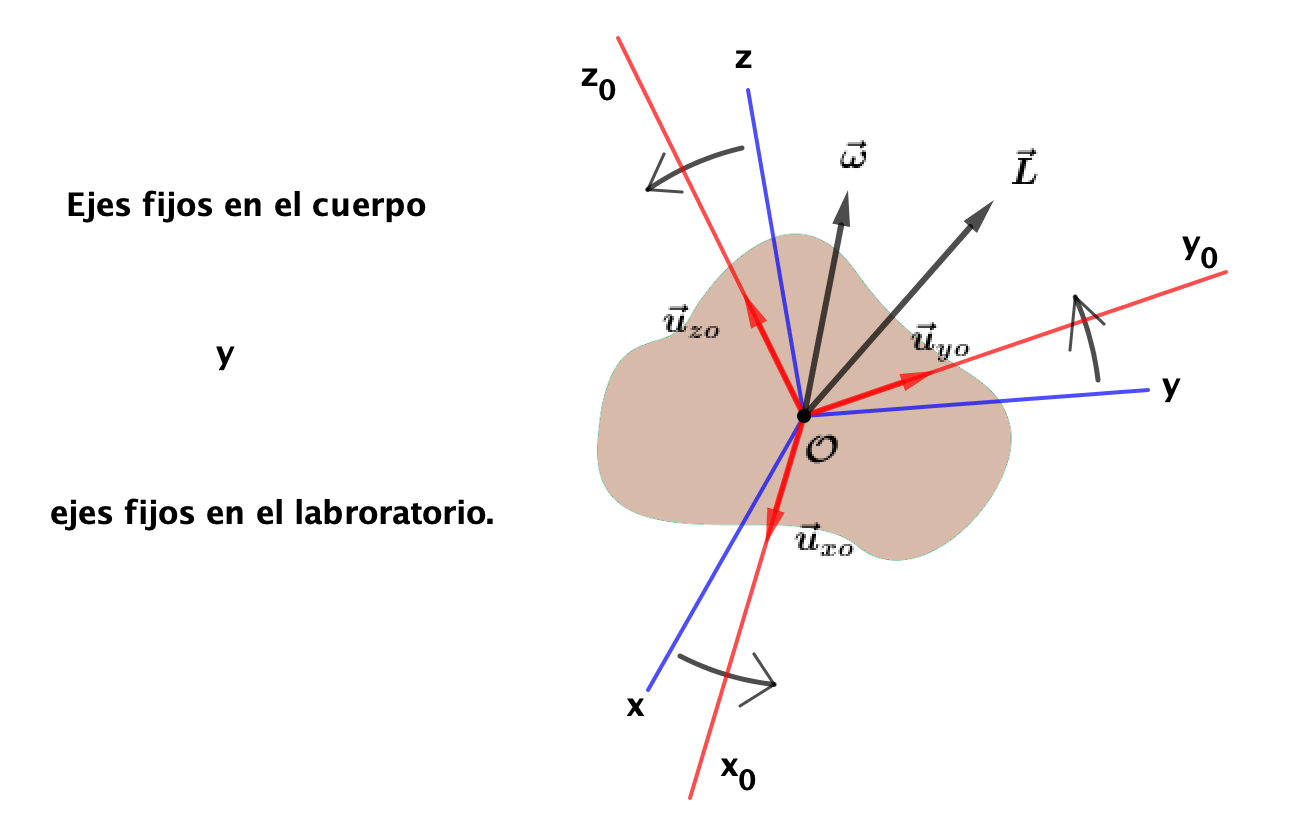
\includegraphics[width=.85\textwidth]{imagenes/imagenes16/T16IM04.png}
\end{figure}

\section{Cálculo del momento de inercia}

Momento de inercia para sistemas de partículas y para objetos extensos.

\begin{equation}
\subrayado{ \ 
I \ = \ \sum_i m_i R_i^2 \ = \ \int R^2 \dd m
\ }	
\end{equation}

Si $\rho$ es a densidad del cuerpo y tenemos una dirección de simetría, $\dd m=\rho \dd z$, tendremos que $I=\int \rho R^2 \dd z$. Si además el cuerpo es homogéneo, $\rho=cte$, podremos escribir $I=\rho \int R^2 \dd z$ y el momento de inercia se reduce a un factor geométrico igual para todos los cuerpos de la misma forma y del mismo tamaño.

Los momentos de inercia respecto a ejes paralelos están relacionados por una fórmula muy simple. Sea $z$ un eje arbitrario y $z_{CM}$ un eje paralelo que pasa por el $CM$ del cuerpo rígido y sea $a$ la separación entre ambos ejes, entonces:

\begin{equation}
\label{Th.Steiner}
\subrayado{ \ \boldsymbol{\ 
I\ =\ I_{CM} + M\ a^2 \ } \ }	 \qquad  \text{Teorema de Steiner}
\end{equation}

\begin{proof}.
\begin{figure}[H]
	\centering
	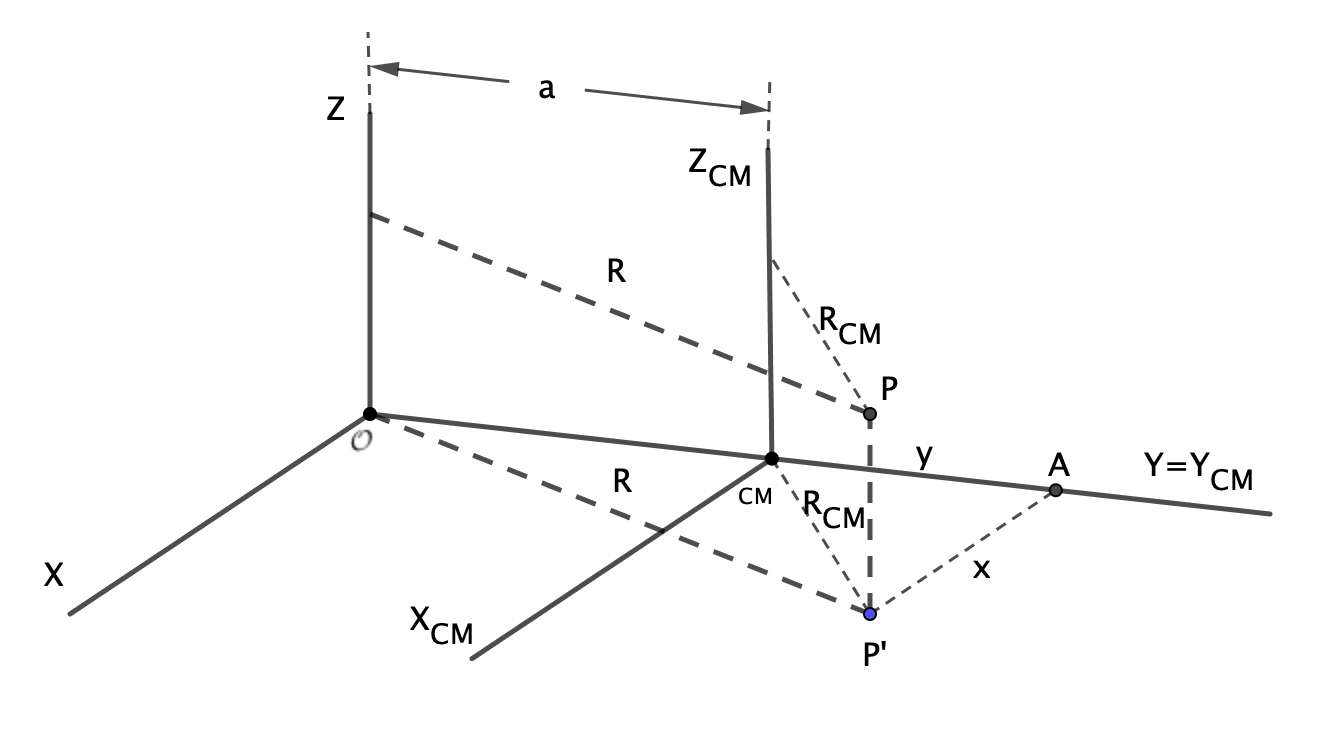
\includegraphics[width=.9\textwidth]{imagenes/imagenes16/T16IM05.png}
\end{figure}
Escogemos los ejes $X_{CM},\ Y_{CM},\ Z_{CM}$ de modo que pasen por el $CM$ del cuerpo y que el eje $Y_{CM}$ se encuentre en el plano $ZZ_{CM}$. Los ejes $X,\ Y,\ Z$ se escogen de modo que $Y$ coincida con $Y_{CM}$. 

Sea $P$ un punto arbitrario del cuerpo rígido de masa $M$. De la figura, obrsevamos que $\overrightarrow{P'A}=x\bot Y_{CM}$ y que $\overrightarrow{\mathcal OA}=y;\ \overrightarrow{\mathcal OCM}=a$

$R^2=x^2+y^2=x^2+(y+a)^2=x^2+y^2+2ay+a^2=R^2_{CM}+2ay+a^2$

ahora, el momento de inercia respecto al eje $Z$ es:

$I=\sum_i mR^2=\sum_i m(R^2_{CM} +2ay+a^2)$

$I=\sum_i mR^2_{CM} \ \textcolor{gris}{(I_{CM})}\ +2a\cancelto{0}{\sum_i my} + a^2\sum_i m \ \textcolor{gris}{ (\sum_i m=M) } \ $

pues $y_{CM}=0=\dfrac{\sum_i my}{\sum m} \to \sum_i my=0$

por lo que:

$$ \boldsymbol{ I \ = \ I_{CM} \ + \ M a^2 }\ ; \quad  \qquad [I]=[ML^2] \ \rightsquigarrow  \ \mathrm{Kg\ m}^2$$
\end{proof}



\begin{figure}[h]
	\centering
	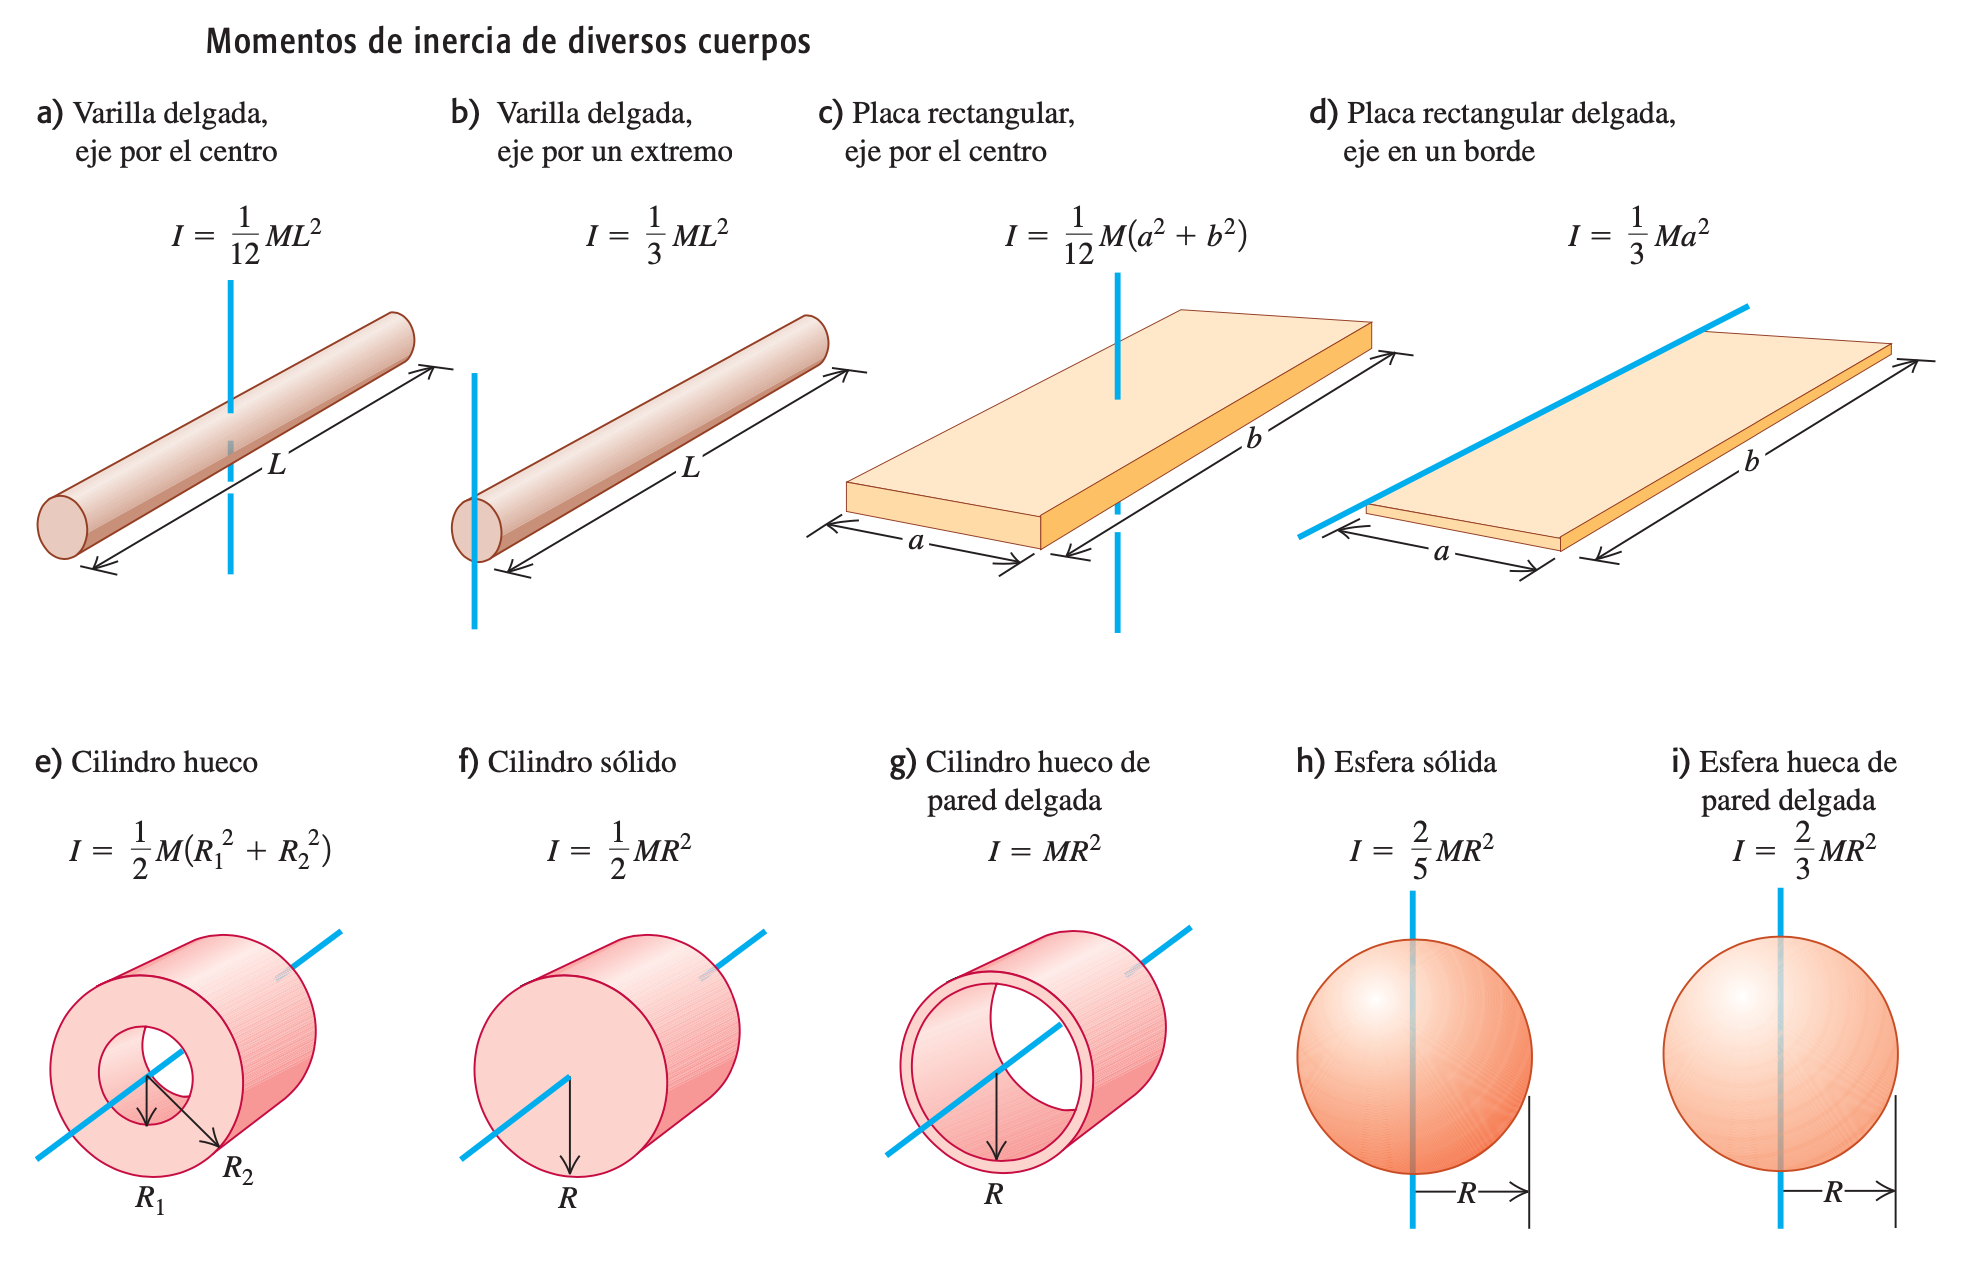
\includegraphics[width=1\textwidth]{imagenes/imagenes16/T16IM06.png}
\end{figure}



\section[Ecuación de movimiento de rotación de un cuerpo rígido]{Ecuación de movimiento de rotación de un cuerpo rígido\sectionmark{Ecuación de movimiento de rotación}}
\sectionmark{Ecuación de movimiento de rotación}
La ecuación básica para discutir el movimiento de rotación del cuerpo rígido es:

$$\displaystyle \boxed{\ \boldsymbol{ \dv{\vec L}{t}=\vec M^{(e)} }\ } \ , \qquad \text{donde}\quad \vec L=\sum_i \vec L_i; \quad \vec M^{(e)}=\sum_i \vec M_i$$ 

------ En primer lugar vamos a estudiar el caso en que el cuerpo rígido rota alrededor de un eje principal que tiene un punto fijo en un sistema de referencia inercial.
$\to \ \displaystyle \vec L=I\vec \omega \to 	\dv{(I\vec \omega)}{t}=\vec M^{(e)}$, 
momento respecto del punto fijo del sistema inercial.

Si el eje permanece fijo respecto al cuerpo rígido, el momento de inercia permanece constante, entonces:

$\displaystyle I\dv{\omega}{t}=M^{(e)} \ \leftrightarrow \ \boldsymbol{ I\alpha=M^{(e)}}$,

donde $\alpha$ es la aceleración angular, $\alpha=\displaystyle \dv{\omega}{t}=\dot{\omega}$. 
Ecuación muy similar al movimiento de una partícula: $ \quad ma=F \quad \sim \quad  I\alpha=M^{(e)}$

Si, p.ej., $\ \vec M^{(e)}=\vec 0 \ \to \ I\vec \omega=\overrightarrow{cte}$ y, si $I=cte ,\ \to \ \vec \omega =\overrightarrow {cte}$.

Es decir, un cuerpo rígido que rota alrededor de un eje principal se mueve con $\vec \omega=\overrightarrow{cte}$
cuando no se aplica $\vec M^{(e)}$. Podemos considerar esta conclusión con \emph{ley de inercia para el movimiento de rotación.}

Si $I\neq cte$, lo es $I \omega=cte$, es decir, si $I$ aumenta (o disminuye), entonces $\omega$ disminuye (o aumenta). Este hecho tiene muchas aplicaciones.

------ Consideremos, ahora, un segundo caso. Veamos cuando el cuerpo rígido no rota respecto a un eje principal.

Sabemos que $\displaystyle \dv{L_z}{t}=M_z^{(e)}$.

Si la orientación del eje es fija con respecto al cuerpo de modo que $I=cte$, tendremos que $\displaystyle I \dv{\omega}{t}= M_z^{(e)} $

Si el eje de rotación no tiene un punto fijo en un sistea inercial, no podemos usar la ecuación $\displaystyle \dv{\vec L}{t}=\vec M^{(e)}$ y tendremos que calcular el momento exterior de fuerzas en el centro de masas del cuerpo, así:

$$ \displaystyle \dv{\vec L_{CM}}{t} \ = \ \vec M_{CM}^{(e)} $$

Si la rotación es alrededor de un eje principal, esta ecuación se convierte en:

$ I_{CM}\displaystyle \dv{\vec \omega}{t}=\vec M_{CM}^{(e)}\ $ y si $\ \vec M_{CM}^{(e)}=\vec 0 \ (*)\ \Rightarrow \ \vec \omega=\overrightarrow{cte} $

$(*)\ $ Cosa que ocurre en el caso de que la única fuerza externa aplicada al cuerpo sea el peso, entonces $\omega$ es constante.

\section{Energía cinética de rotación}

Energía cinética de un sistema de partículas $\ \displaystyle \mathcal E_c=\sum_i \dfrac 1 2 m_i v_i^2$

En el caso de un cuerpo rígido rotando con $\omega$ entorno a un eje, $v_i=\omega R_i$, con $R_i$ la distancia al eje de rotación, por lo que:

$\displaystyle \boldsymbol{ \mathcal E_c=} \ \sum_i \dfrac 1 2 m_i v_i^2=\sum_i \dfrac 1 2 m_i R_i^2 \omega^2 =\dfrac 1 2 \left( \sum_i m_i R_i^2 \right) \omega^2 \ \boldsymbol{ =\dfrac 1 2 I \omega^2 }$

Cuando la rotación se produce entrono a un eje principal de inercia, se tiene que $\ L=I\omega \to \omega=\dfrac L I \ $ y la energía cinética es

$\boldsymbol{ \mathcal E_c=}\  \dfrac 1 2 \  I \   \dfrac {L^2} {I^2} = \ \boldsymbol{ \dfrac{L^2}{2I}}$

Podemos obtener una expresión más general usando las componentes de $\vec \omega$ a lo largo de los ejes principales $x_0, y_0, z_0$. El resultado es:

$\mathcal E_c=\dfrac 1 2 \left( I_1 \omega^2_{x_0}+I_2 \omega^2_{y_0}+I_3 \omega^2_{x_0}\right)$.

Como $\vec L=\vec u_{x_0} \ I_1 \omega_{x_0}+\vec u_{y_0} \ I_2 \omega_{y_0} +\vec u_{z_0} \ I_3 \omega_{z_0}$,

$\mathcal E_c= \dfrac 1 2 \left(  \dfrac{L^2_{x_0}}{I_1}+  \dfrac{L^2_{y_0}}{I_2}+  \dfrac{L^2_{z_0}}{I_3} \right)$

Un caso interesante es cuando un cuerpo presenta simetría de revolución (como en las rotaciones moleculares), por ejemplo entorno a $x_0$, de modo que $I_1=I_2$

$\mathcal E_c=\dfrac 1 2 \left[ \dfrac 1 {I_1} ( L^2_{x_0}+L^2_{y_0} \ )+\dfrac 1 {I_3} L^2_{z_0}  \right]$

Consideremos ahora que el eje de rotación del cuerpo rígido pasa por el $CM$ y, además de rotar, tiene un movimiento relativo de traslación respecto al observador.

$\mathcal E_c=\dfrac 1 2 M V^2_{CM} \ + \ \mathcal E_{C,CM}$

En el cuerpo rígido, $\dfrac 1 2 M v_{CM}^2 = \mathcal E_{c,\text{traslación}} \to \mathcal E_{C,CM}$ es la energía cinética de rotación respecto al $CM$. Podemos escribir:

\vspace{-3mm} $$\mathcal E_c= \dfrac 1 2 M V^2_{CM}+ \dfrac 1 2 I_{CM} \omega^2$$

\vspace{-3mm} Como las distancias entre las partículas internas del cuerpo rígido no cambian, $\mathcal E_{P,int}=cte$ y nos las consideramos al explicar el intercambio energético del cuerpo rígido con sus alrededores:

$$\mathcal E_c \ - \mathcal E_{c,0} \ = \ W_{ext}$$

Para el caso de fuerzas conservativas, $\ W_{ext}=(\ \mathcal E_{p}-\mathcal E_{p,0}\ )_{ext}$

por lo que $\ \mathcal E_c+\mathcal E_p=(\mathcal E_c+\mathcal E_p)_0$

Con lo que $\boxed{\  \subrayado{ \  \boldsymbol{E=\dfrac 1 2 Mv^2_{CM} + \dfrac 1 2 I_{CM} \omega^2 + \mathcal E_p = cte} \ } \ }$

Si el cuerpo cae bajo la acción de la fuerza gravitatoria, $\mathcal E_p=Mh$, donde $h$ es la altura del $CM$ respecto a un plano horizontal de referencia.

Si hay fuerzas no conservativas (p.ej., fuerzas de fricción):  $\ W_{ext}=\mathcal E_{p,0}-\mathcal E_p+W'$, donde $W'$ es el trabajo efectuado por las fuerzas no conservativas. En este caso:

$$(\mathcal E_c+\mathcal E_p)\ - \ (\mathcal E_c+\mathcal E_p)_0\ =\ W'$$


\section{Problemas}
\begin{prob}

\begin{multicols}{2}.

Calcular el momento angular de la figura adjunta, que consta de 2 esferas de masa $m$ cada una, montadas sobre brazos de longitud $R$ conectados a un eje que les permie rotar a su alrededor. 	
\begin{figure}[H]
	\centering
	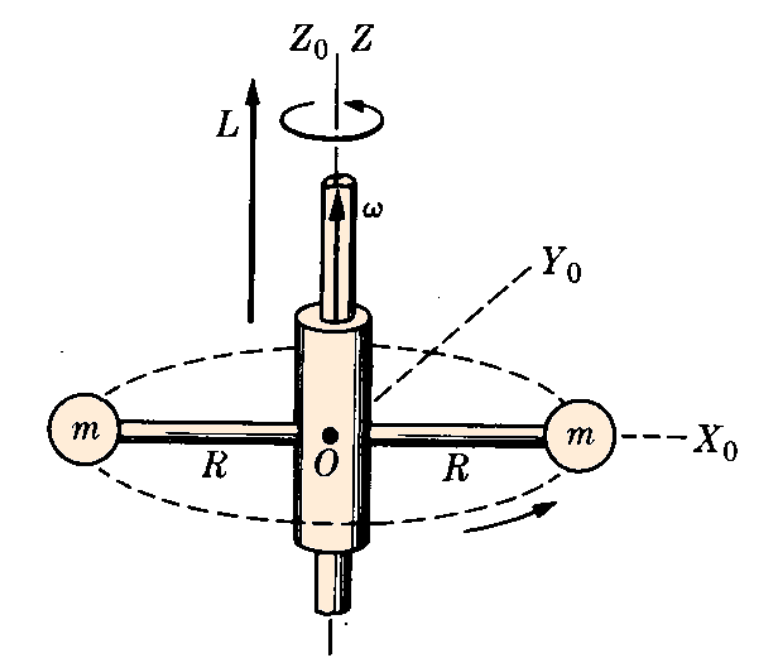
\includegraphics[width=.4\textwidth]{imagenes/imagenes16/T16IM08.png}
\end{figure}
\end{multicols}	
\end{prob}

Cada esfera describe un círculo de radio $R$, con velocidad $v=\omega R$ alrededor del eje $Z$ de giro. Respecto a $\mathcal O$, el momento angular de cada esfera es $\vec L=mR^2\omega \ \vec u_z$ y el momento total $\vec L=2mR^2\omega \ \vec u_z=2mR^2 \ \vec \omega$, el sistema rota entorno a su eje principal $Z_0=Z$.

En estas condiciones, $L=I\omega \ to \ I=2mR^2$ es el momento principal de inercia.


\begin{prob}
Calcular el momento de inercia de una varilla delgada homogénea respecto a un eje perpendicular a la varilla que pase por  a)  un extremo	, y b) el centro.
\end{prob}
\begin{figure}[H]
	\centering
	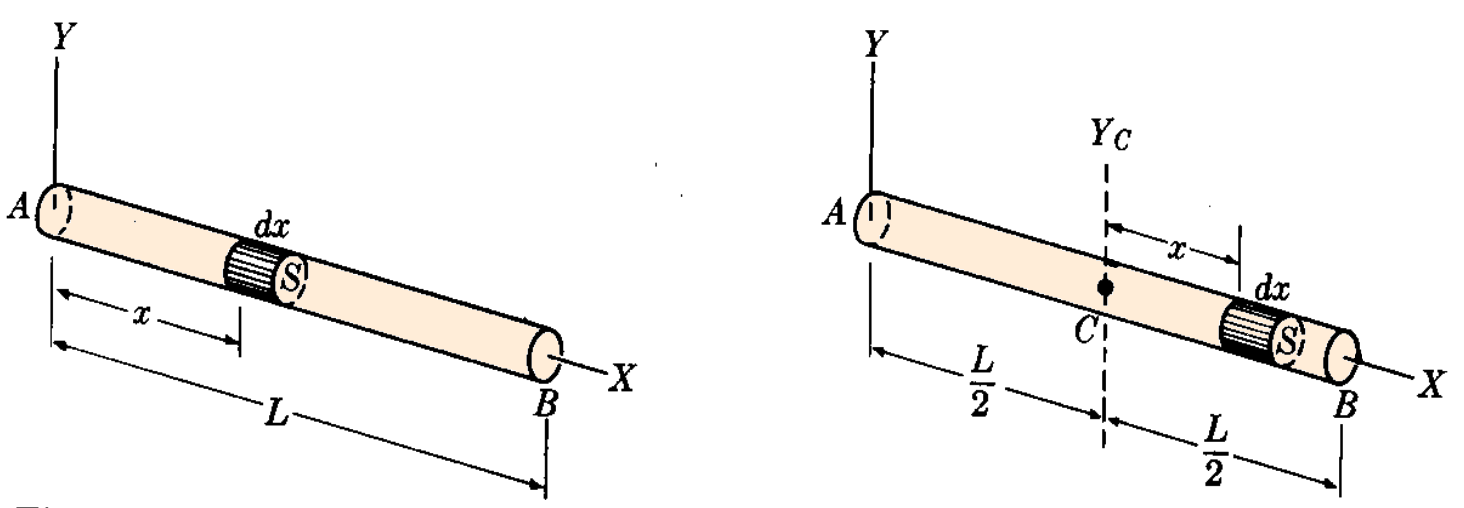
\includegraphics[width=.9\textwidth]{imagenes/imagenes16/T16IM09.png}
\end{figure}

--- a) Sea $L$ la longitud de la varilla y $S$ su superficie, que supondremos muy pequeña. Dividimos la varilla en pequeños segmentos, a distancia $x$ del eje de rotación $A$, de espesor $\dd x$ y volumen $\dd V=S\dd x$, con ello:

$\displaystyle I_A=\displaystyle \int_0^L \lambda x^2 (S\dd x)=\lambda S \int_O^L x^2 \dd x= \dfrac 1 3 \lambda S L^3$

Donde hemos llamado $\lambda$ a la densidad lineal de masa de la varilla, que por ser homogénea, $\lambda=\dfrac M{LS}$, con lo que
$\ I_A=\dfrac 1 3 \dfrac{M}{LS} SL^3=\dfrac 1 3 M L^2$

--- b) Para calcular el momento de inercia respecto a un eje paralelo que pasa por su centro, que es el $CM$ del cuerpo, como $Y\; || \; Y_C$, usaremos el Teorema de Steiner:
$I_A=I_{CM}+M\left( \dfrac 1 2 L \right)^2$, pues, en este caso, $a=\dfrac 1 2 L$ 

$\dfrac 1 3 M L^2=I_{CM}+\dfrac 1 4 M L^2 \ \to \ I_{CM}=\dfrac{1}{12}ML^2$

\textcolor{gris}{También podríamos haber llegado a este resultado integrando ahora desde $-L/2$ hasta $+L/2$: $\ \displaystyle I_{CM}=\lambda S \int_{-L/2}^{L/2}x^2 \dd x=\dfrac {M}{LS} S \left[ \dfrac {x^3}{3} \right]_{-L/2}^{L/2} = \dfrac {1}{12} ML^2$}

\textcolor{gris}{Incluso podríamos haber obtenido $I_{CM}$ suponiendo la varilla dividida en dos, con masas $M/2$ y longitud $L/2$ cada una de ellas girando sobre un extremo, $C$, así,
$\ I_{CM}=2\ \dfrac 1 3 \ (M/2)\ (L/2)^2 = \dfrac 1 {12} ML^2$}


\vspace{10mm} %*****************************************
\begin{prob}
Calcular el momento de inercia de una aro respecto de un eje que pasa por uno de sus diámetros.	
\end{prob}

\begin{multicols}{2}
Anillo homogéneo, densidad lineal de masa:

$\lambda=\dfrac {M}{2\pi R}$

$ \dd m=\lambda \dd l=\lambda R\dd l =\dfrac {M}{2\pi \cancel{R}}\cancel{R}\dd \theta$

$x=R\sin \theta$

$I=\displaystyle \int_M x^2 \dd m$
\begin{figure}[H]
	\centering
	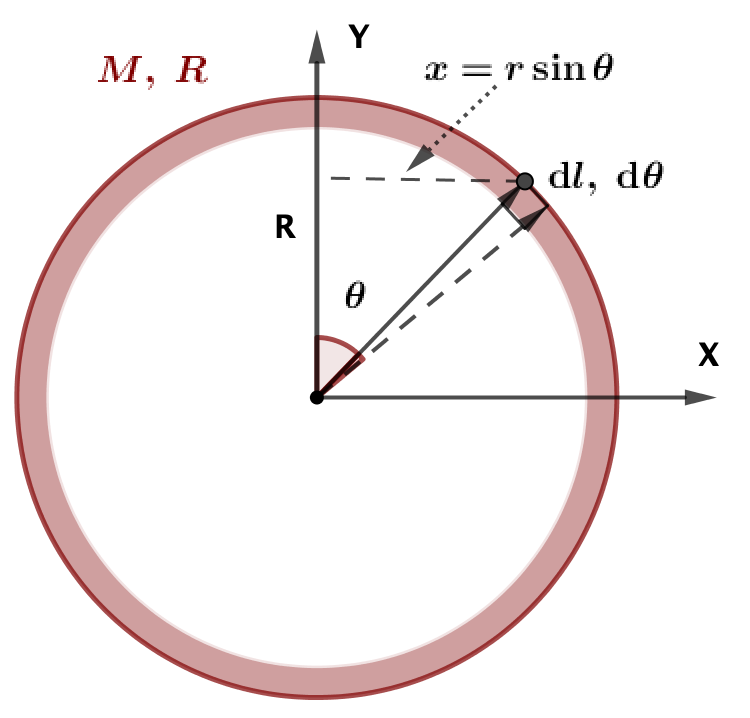
\includegraphics[width=.25\textwidth]{imagenes/imagenes16/T16IM15.png}
\end{figure}	
\end{multicols}

$\displaystyle I=\int_0^{2\pi} (R\sin \theta)^2 \dfrac {M}{2\pi} \dd \theta
= \dfrac{MR^2}{2\pi} \int_0^{2\pi} \sin^2 \theta \dd \theta$

\small{$\begin{cases} \ \ \sin^2 \theta+\cos^2\theta &=1 \\ -\sin^2\theta+\cos^2\theta &=\cos 2\theta \end{cases} \to 2\sin^2\theta=1-\cos 2\theta;\quad \sin^2\theta=\dfrac 1 2 -\dfrac 1 2 \cos 2 \theta$}

\normalsize{$\displaystyle I=\dfrac{MR^2}{2\pi} \left[ \dfrac 1 2 \int_0^{2\pi} \dd \theta - \dfrac 1 {2\ \boldsymbol{2}}\int_0^{2\pi}\boldsymbol{2}\cos 2\theta \dd \theta \right] $}$=\displaystyle \dfrac{MR^2}{2\pi} \left[ \left(\theta \right)_0^{2\pi}-\dfrac 1 4 \left( \sin 2\theta \right)_0^{2\pi} \right] $

$\displaystyle I=\dfrac{MR^2}{2\pi} \left[ 2\pi-\dfrac 1 4 \cdot 0 \right]=
\dfrac{MR^2}{\cancel{2\pi}} \cancel{2\pi}=MR^2$

\vspace{10mm} %*****************************************
\begin{prob}
Calcular el momento de inercia de un disco homogéneo con respecto a un eje perpendicular que pasa por su centro.	
\end{prob}

\vspace{10mm} %*****************************************
\begin{multicols}{2}
Dada la simetría del problema, usaremos con elemento de volumen $\dd V$ un anillo de radio $r$ y espesor $\dd r$. Sea $h$ el espesor del disco, que suponemos muy pequeño. La densidad superficial de masa es $\sigma=\dfrac M{Sh}=\dfrac{M}{h\pi R^2}$ y la masa de anillo, situado a distancia $r$ del eje de giro, será:

$\dd m =\sigma \dd V = \sigma h \dd S= \sigma h 2\pi r \dd r$
\begin{figure}[H]
	\centering
	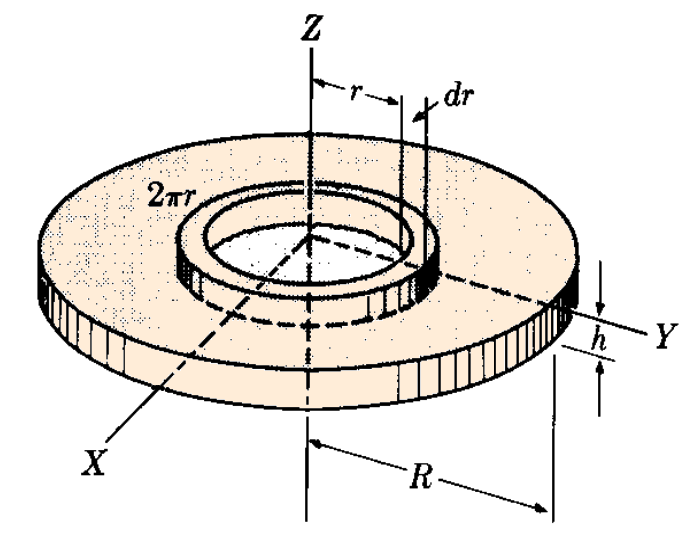
\includegraphics[width=.4\textwidth]{imagenes/imagenes16/T16IM10.png}
\end{figure}
\end{multicols}

$I=\displaystyle \int_0^R \sigma h \ r^2 \ 2\pi r \dd r=2\pi \sigma h \int_0^R r^3 \dd r=\dfrac 1 2 \pi \sigma h R^4 = \dfrac 1 2 \pi \dfrac {M}{\pi R^2 h} h R^4 $

Por lo que, finalmente, $\ I=\dfrac 1 2 M R^2$

\begin{prob}
Calcular el momento de inercia de una esfera maciza respecto de un eje que pasa por su centro.	
\end{prob}

Resolveremos el problema de dos formas distintas.

------ \underline{Método I}:  Primero calcularemos el momento de inercia de una esfera hueca para, después, considerar la esfera maciza como una serie de cáscaras de esferas huecas, como una cebolla.

\vspace{35mm} %****************************************************
\begin{multicols}{2}
La esfera hueca de masa $M$ y radio $R$ tiene una densidad superficial de masa: $\sigma=\dfrac{M}{4\pi R^2}$

El elemento de área mostrado tiene longitud $2\pi x$ y anchura $R\dd \theta$, por lo. que $\dd S= 2\pi x R \dd \theta$

$I=\displaystyle \int_M x^2 \dd m=\int_M x^2 \sigma \dd S=\int_M x^2 \dfrac {M}{4\pi R^2} 2 \pi x R \dd \theta =\dfrac{M}{2R}\int_M x^3 \dd \theta= \dfrac {M}{2R}\int_{-\pi/2}^{\pi/2}R^3 \cos^3 \theta \dd \theta$
\begin{figure}[H]
	\centering
	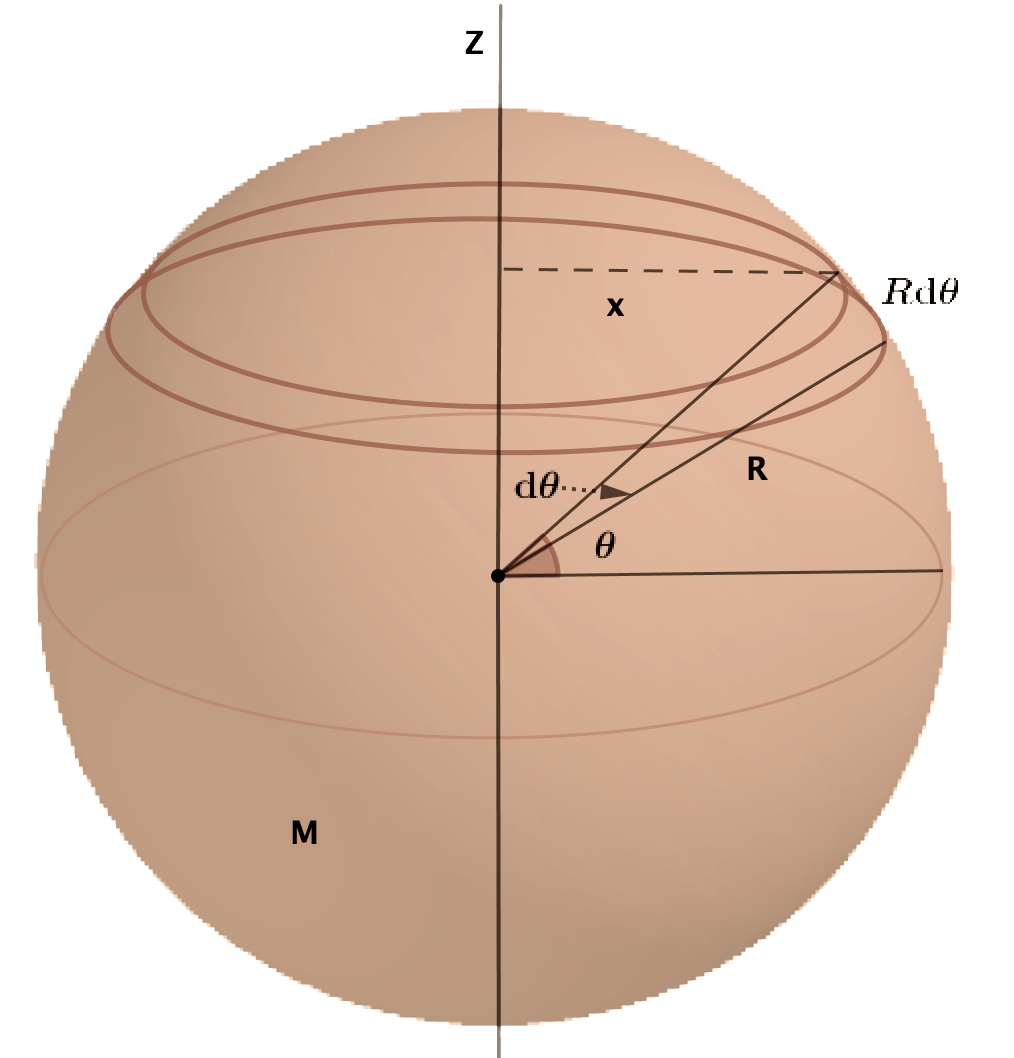
\includegraphics[width=.35\textwidth]{imagenes/imagenes16/T16IM16.png}
\end{figure}
\end{multicols}

\textcolor{gris}{\footnotesize{$\displaystyle \int \cos^3(\theta)\dd \theta = \int \cos \theta (1-\sin^2 \theta) \dd \theta = \int  \cos \theta \dd \theta - \int \sin^2 \theta \cos \theta \dd \theta = \sin \theta - \dfrac {\sin^3 \theta}{3} + \mathcal C$}}\normalsize{.}

$\displaystyle I=\dfrac{MR^2}{2} \left[\eval{\sin \theta - \dfrac {\sin^3 \theta}{3}}_{-\pi/2}^{\pi/2}\right.=\dfrac 2 3 MR^2$


\begin{multicols}{2}
Vamos ahora a por el momento de inercia de la esfera hueca que consideramos como formada por capas de esferas huecas a modo de capas de cebolla. Las capas estarán situadas a distancia $r$ del centro, de espesor $\dd r$ y con momento de inercia $\dd I=\dfrac 2 3 r^2 \dd m$. 

$r$ variará desde $0$ hasta $R$.

Para la esfera homogénea, 
$\rho=\dfrac {M}{\frac 4 3 \pi R^3}$
\begin{figure}[H]
	\centering
	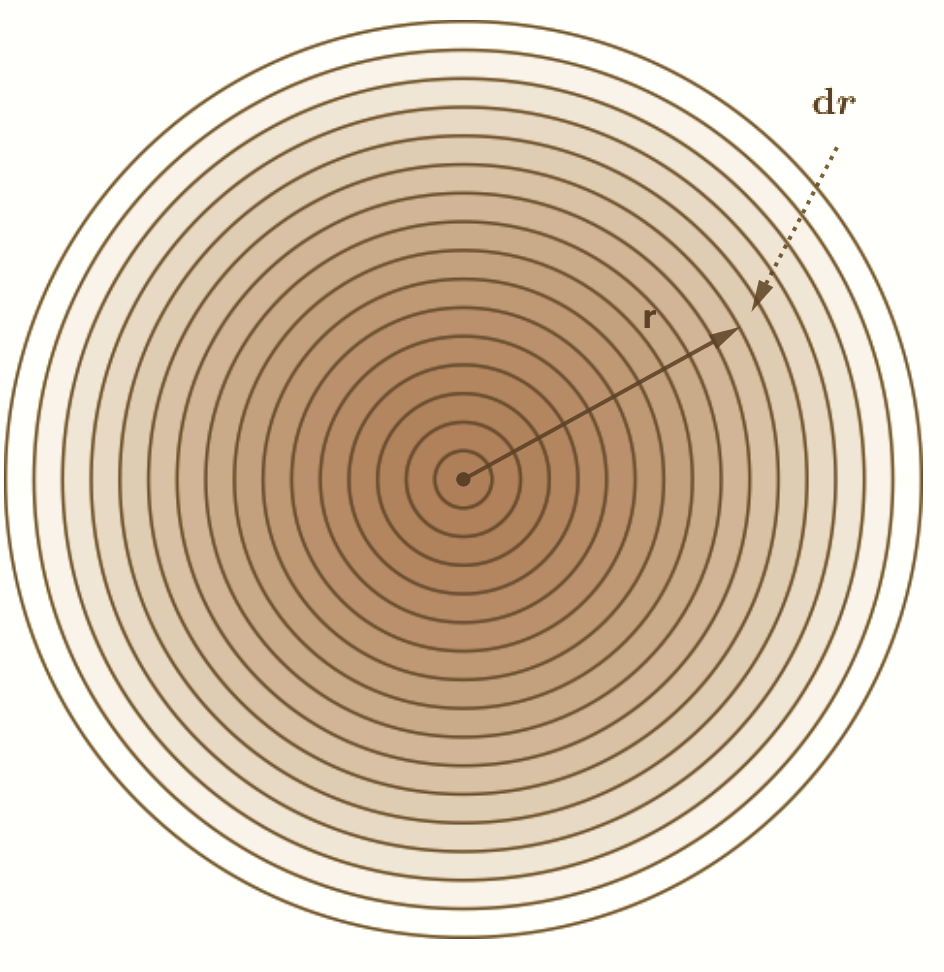
\includegraphics[width=.3\textwidth]{imagenes/imagenes16/T16IM17.png}
\end{figure}
\end{multicols}

$V=\dfrac 4 3 \pi r^3 \to \dd V=4\pi r^2 \dd r;\qquad \dd m= \rho \dd V$

$\displaystyle I=\int_M \dd I =\int_M \dfrac 2 3 r^2 \dd m = \int_M \dfrac 2 3 r^2 \rho  4  \pi r^2 \dd r = \dfrac {8\pi}{3}\rho \int_O^R r^4 \dd r$

$\displaystyle I=
\dfrac {8\pi}{3} \dfrac {M}{\frac 4 3 \pi R^3} \left[ \eval{\dfrac {R^5}{5}}_0^R \right. = 
\dfrac {8\cancel{\pi}}{\cancel{3}} \dfrac{M}{\dfrac{4}{\cancel{3}}\cancel{\pi} R^3} \dfrac{R^5}{5} = \dfrac 2 5 M R^2$



------ \underline{Método II}: Consideraremos la esfera maciza formada por una serie de discos de espesor diferencial girando sobre un eje perpendicular a ellos que pasa por su centro ($I_{disco}=\frac 1 2 MR^2$).


Consideremos uno de estos discos, a altura $z$ desde el centro de la esfera, con radio r y espesor $\dd r$. Como muestra la figura.

Su momento de inercia será $\dd I=\dfrac 1 2 r^2 \dd m$

La masa de cada disco es:
$\ \dd m=\rho \dd V = \rho \pi r^2 \dd z;$
$\quad \rho=\dfrac{M}{\frac 4 3 \pi R^3}=\dfrac{3M}{4\pi R^3}$

\vspace{40mm} %***************************************************

\begin{multicols}{2}
Luego, $\dd I=\dfrac 1 2 r^2 \dfrac{3M}{4\pi R^3} \pi r^2 \dd z= \dfrac{3M}{8R^3}r^4 \dd z$

$\displaystyle I= \dfrac{3M}{8R^3} \int_{-R}^{R} r^4 \dd z;\qquad r^2+z^2=R^2 \to $

$\displaystyle I=\dfrac{3M}{8R^3} \left[ \eval{R^2x-\dfrac{x^3}{3}}_{-R}^{R}\right. = \dfrac 2 5 MR^2$
\begin{figure}[H]
	\centering
	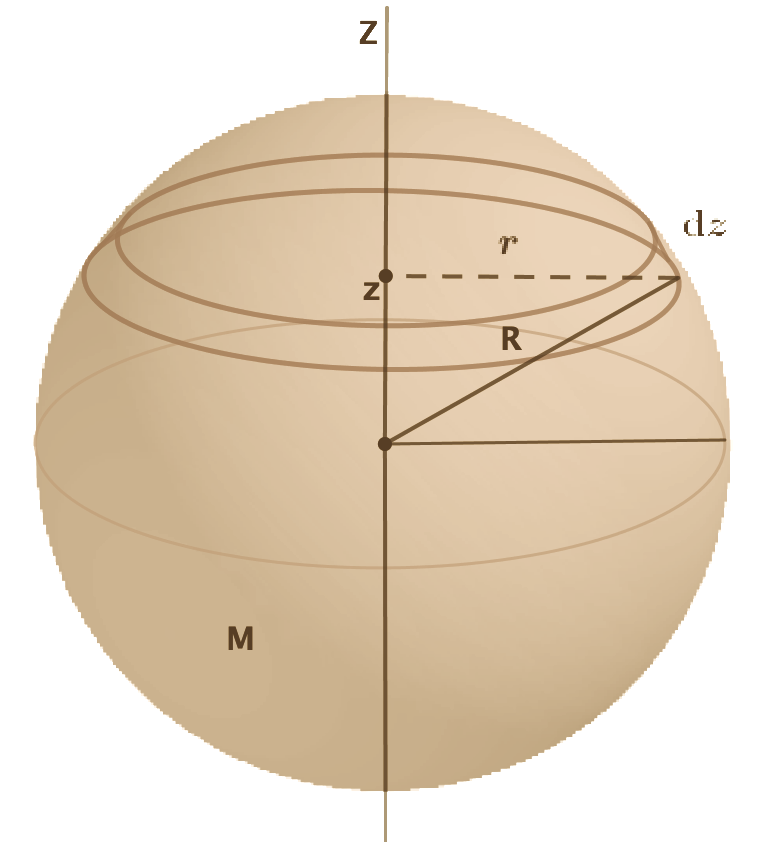
\includegraphics[width=.3\textwidth]{imagenes/imagenes16/T16IM18.png}
\end{figure}
\end{multicols}

\begin{prob}
Un disco de $0.5\ \mathrm{m}$  de radio y $20\ \mathrm{kg}$ de masa	puede rotar libremente alrededor de un eje horizontal fijo que pasa por su centro. Se aplica una fuerza de $F=9.8\ \mathrm{N}$ tirando de una cerda atada al borde del disco. Encontrar la aceleración angular del disco y su velocidad angular al cabo de $2\ \mathrm{s}$
\end{prob}


\begin{multicols}{2}
$\quad$

Las únicas fuerzas externas sobre el disco son su peso $Mg$, la fuerza de la cuerda $F$, ambas hacia abajo y las reacciones $F'$ en los soportes del montaje. $ZZ'$ es un eje principal.
\begin{figure}[H]
	\centering
	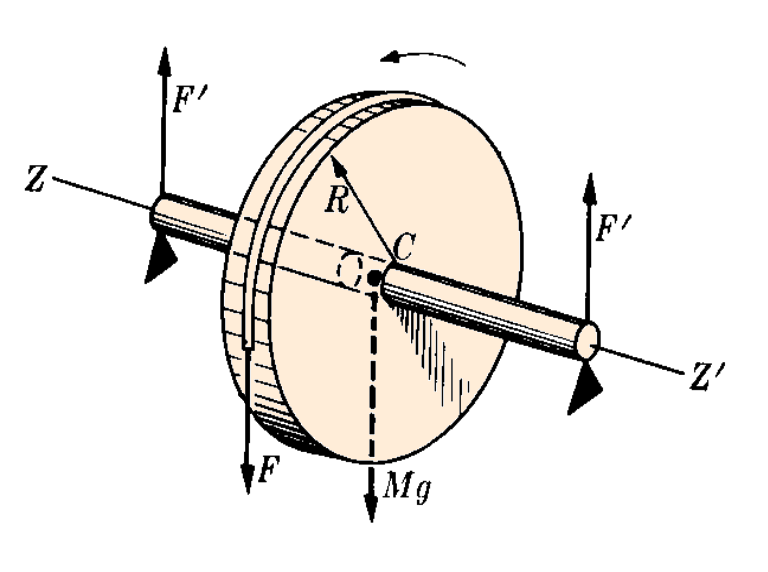
\includegraphics[width=.5\textwidth]{imagenes/imagenes16/T16IM11.png}
\end{figure}
\end{multicols}



Calculamos el momento de las fuerzas respecto al $CM$, el correspondiente al peso es cero pues lo es su distancia a $C$. El de las fuerzas $F'$ combinadas también es cero (regla sacacorchos), con lo que $M^{(e)}=FR$.

Como hemos visto antes, el momento de inercia de un disco de masa $M$ y radio $R$ girando alrededor de un eje perpendicular que pasa por el entro es $I=\dfrac 1 2 MR^2$, tendremos que: 

$M=I\alpha \ \to \ FR=\dfrac 1 2 M R^2 \alpha \ \to \ \alpha=\dfrac{2F}{MR}=cte$

Tenemos un movimiento circular uniformemente acelerado: $\omega=	alpha t$. Sustituyendo los datos del problema:

$\alpha = 1.96 \ \mathrm{rad\ s}^{-2};\quad \omega (t=2)=3,92 \mathrm{rad\ s}^{-1}$

Como $C$ está fijo, la reacción en los soportes es: $2F'-Mg-F=0 \ \to \ F'=102,9\ \mathrm{N}$

\vspace{40mm} %*********************************************
\begin{prob}
\begin{multicols}{2}
$\quad$

Calcular la aceleración angular del sistema de la figura adjunta para un cuerpo de $1\ \mathrm{kg}$ de masa. Los datos del disco son los mismos que los del problema anterior, se trata de un disco de $0.5\ \mathrm{m}$  de radio y $20\ \mathrm{kg}$ de masa	que puede rotar libremente alrededor de un eje horizontal fijo que pasa por su centro.
\begin{figure}[H]
	\centering
	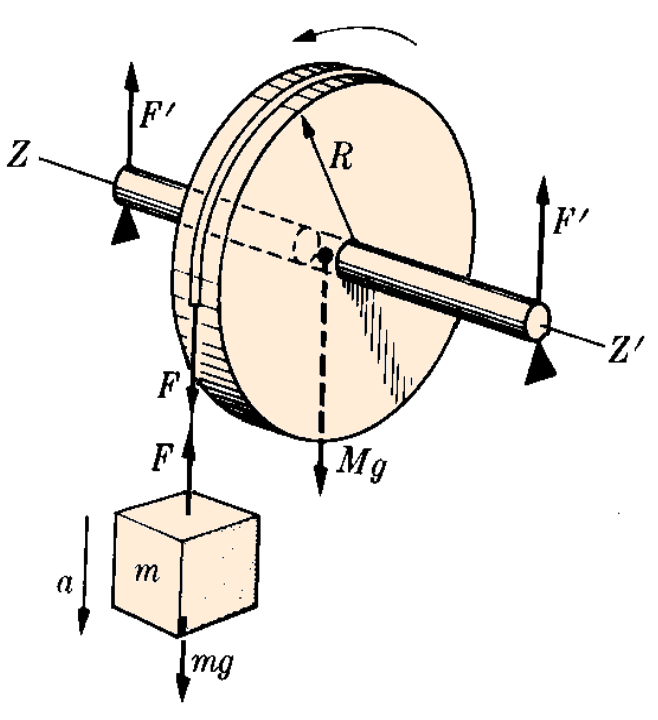
\includegraphics[width=.35\textwidth]{imagenes/imagenes16/T16IM12.png}
\end{figure}	
\end{multicols}
\end{prob}

$m=1\ \mathrm{kg} \ \to \ F=9.8\ \mathrm{N}$, como en el problema anterior. Parece que el resultado debe ser el mismo que en el problema anterior, pero no es cierto: la masa al caer ejerce una fuerza $F$ hacia abajo sobre el disco, pero el disco ejerce una fuerza $F$ hacia arriba por acción-reacción. Como $m$ cae con $MRUA$, la fuerza total sobre ella no puede ser cero, por lo que será $mg-F$, y el momento también será menor.

Ecuación de movimiento de la masa $m$: 

$\ mg-F=ma=MR\alpha$

Ecuación de movimiento del disco:

$(I=\frac 1 2 MR^2)$: $\ I\alpha=FR; \ \frac 1 2 M R^{\cancel{2}} \alpha=F\cancel{R}$

Eliminando $F$ de ambas ecuaciones, se encuentra 

$\alpha=\dfrac{mg}{\left( m+\dfrac 1 2 M \right)R}=1.8 \ \mathrm{rad\ s}^{-2}$

La aceleración hacia abajo de $m$ es 

$\ a=R\alpha=\dfrac{mg}{\left( m+\dfrac 1 2 M \right)}=0.90 \ \mathrm{m\ s}^{-2} < 9.8 \ \mathrm{m\ s}^{-2}$ que sería la que sentiría $m$ en caída libre.

La reacción $F'$ en los soportes se puede calcular como en el problema anterior. Al estar $C$ fijo:

$2F'+F-F-Mg-mg=0 \ \to \ F'=102,9\ \mathrm{N}$

\begin{prob}
\begin{multicols}{2}
Determinar la aceleración angular del disco y la aceleración hacia abajo del $CM$ de la figura adjunta.

Los datos del disco son los mismos que los del problema anterior, se trata de un disco de $0.5\ \mathrm{m}$  de radio y $20\ \mathrm{kg}$ de masa	que puede rotar libremente alrededor de un eje horizontal fijo que pasa por su centro.
\begin{figure}[H]
	\centering
	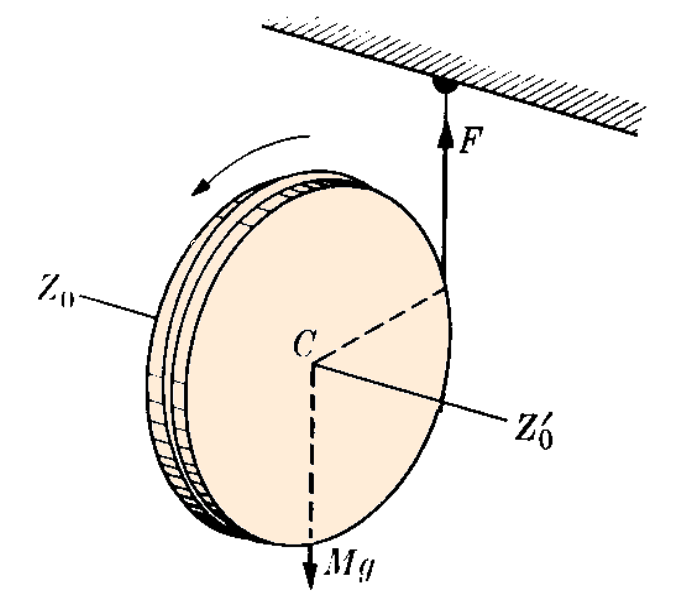
\includegraphics[width=.35\textwidth]{imagenes/imagenes16/T16IM13.png}
\end{figure}	
\end{multicols}
\end{prob}

$ZZ_0$ es el eje principal de rotación pero en este caso, al contrario que en los dos anteriores, el $CM$ no está fijo, por lo que la ecuación a usar ahora es:
$\displaystyle \dv{\vec L}{t}=\vec M^{(e)}_{CM}$. 
El movimiento es como el de un ``yo-yo''.

El momento de $Mg$ respecto a $CM$ es cero, por lo que la rotación del disco vienen dada por $\ I\alpha=FR$, con $I=\frac 1 2 MR^2$, entonces:

$\ I\alpha=FR; \ \frac 1 2 M R^{\cancel{2}} \alpha=F\cancel{R} \ \to \ F=\dfrac 1 2 M R \alpha$

El movimiento del $CM$ hacia abajo se realiza con una aceleración $a=R\alpha$

$F$ es la reacción de la cuerda que sujeta el disco deslizante y la fuerza resultante sobre él es: $mg-F$ y según la segunda de Newton $F_{res}=Ma$, tendremos que $\ Mg-F=Ma=MR\alpha$

Sustituyendo el valor de $F$ encontrado antes, $ \ \cancel{M}g-\dfrac 1 2 \cancel{M}R\alpha=\cancel{M}R\alpha \to g=\dfrac 3 2 R\alpha \to \alpha =\dfrac{2g}{3R}=13.16\ \mathrm{rad\ s}^{-1}$

La aceleración hacia abajo del $CM$ será $a=R\alpha=\dfrac 2 3 g= 6.53 \  \mathrm{m\ s}^{-1}$, menor que en caída libre e independiente del tamaño $R$ u de la masa $M$ del disco.

\begin{prob}
Una esfera, un cilindro y un aro, todos de la misma masa y el mismo radio, ruedan hacia abajo por un plano inclinado partiendo de una altura $y_0$. Encontrar la velocidad con que llegan a la base del plano.	
\end{prob}

\begin{multicols}{2}
Las fuerzas que actúan sobre el cuerpo rodante son, su peso $Mg$, la reacción normal del plano $N$ y la fuerza de rozamiento $F$. Podemos hacer un estudio dinámico o energético, que es el que haremos en este caso.
\begin{figure}[H]
	\centering
	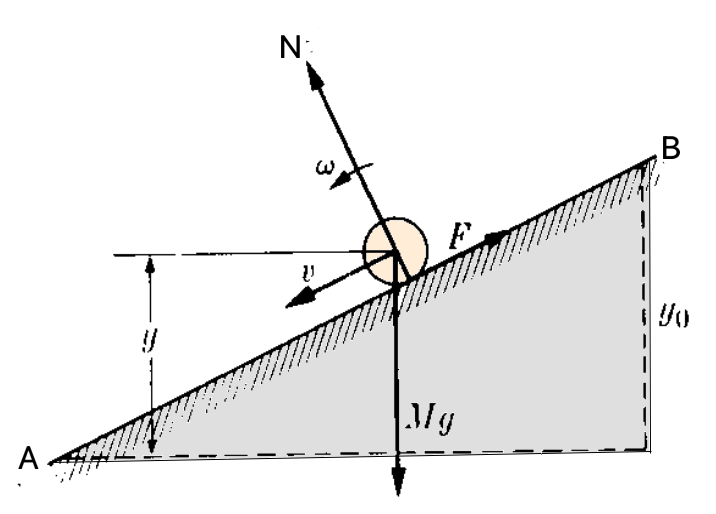
\includegraphics[width=.35\textwidth]{imagenes/imagenes16/T16IM14.png}
\end{figure}	
\end{multicols}
Aplicando el principio de conservación de la energía:

$B=\dfrac 1 2 Mv^2_{CM} + \dfrac 1 2 I_{CM} \omega^2 + \mathcal E_p = cte.\quad$ En $B,\  E_B=Mgy$

En cualquier punto intermedio, el $CM$ se mueve con velocidad de traslación $v$ y el cuerpo rota respecto del $CM$ con velocidad angular $\omega$, ambas relacionadas por $v=\omega R$ y la energía será:

$E=\dfrac 1 2 Mv^2_{CM} + \dfrac 1 2 I_{CM} \omega^2 + Mgy$ 
Al final delmplano, en $A,\ y=0$ y $E_A=\dfrac 1 2 Mv^2_{CM} + \dfrac 1 2 I_{CM} \omega^2$ 

$E_A=E_B \ \to \ \dfrac 1 2 Mv^2_{CM} + \dfrac 1 2 I_{CM} \omega^2=Mgy_0$

Si en lugar de un cuerpo rodante tuviésemos un cuerpo que se desliza sin rodar ($\omega=0$), no tendríamos que incluir la energía cinética de rotación y el resultado sería $\dfrac 1 2 Mv^2_{CM} =Mgy_0$, como el de una partícula simple. El movimiento de rotación hace que el de traslación sea más lento. En un cuerpo rodante, la energía inicial ha de invertirse en energía de rotación y de traslación

Sustituyamos ahora $I_{CM}$ por los tres problemas propuestos, esfera, cilindro y aro ($E,\ C,\ A$). En cualquier tabla de. momento de inercia encontramos que

$I_E=\dfrac 2 5 MR^2;\quad I_C=\dfrac 1 2 MR^2;\quad I_A=MR^2$, sustituyendo y desejando,

$v_E^2=\dfrac {10}{7}gy_0;\qquad v^2_D=\dfrac 4 3 gy_0;\qquad V^2_A=gy_0$ 

En la partícula simple, $v^2=2gy_0$. Así, el cuerpo más rápido es la esfera, le sigue el cilindro y, por último, el aro.

Este resultado indica que la velocidad de un cuerpo que desciende sobre una pendiente no depende ni de su masa ni de sus dimensiones sino solamente de su forma.

\begin{prob}
Dos niños, cada uno de $25\ \mathrm{kg}$ de masa están sentados en extremos opuestos de una plancha horizontal de $2.6\ \mathrm{kg}$ de masa y $2.6\ \mathrm{m}$ de longitud. La plancha está girando a $5\ \mathrm{rpm}$ 	sobre un pivote situado en su centro. ?`Cuál es la velocidad angular con que gira el sistema cuando ambos niños se acercan $60\ \mathrm{cm}$ cada uno hacia el centro? ?`Cuál es el cambio en la energía cinética de rotación del sistema?
\end{prob}

$m=25\ \mathrm{Kg};\quad M=10\ \mathrm{kg};\quad L=2.6\ \mathrm{m};\quad d=1.3\ \mathrm{m}; \quad d'=0.9\ \mathrm{m}$

$\omega= 5 \ \mathrm{rpm}=5\dfrac {2\pi}{60} = \dfrac \pi 6 =0.52 \ \mathrm{rad\ s}^{-1}$

\begin{figure}[H]
	\centering
	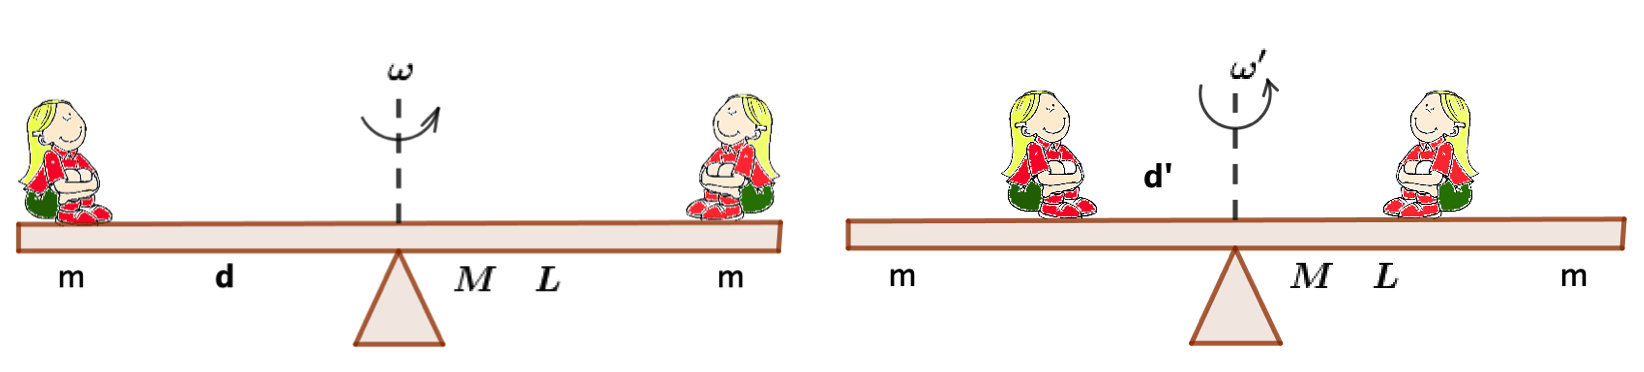
\includegraphics[width=.8\textwidth]{imagenes/imagenes16/T16IM19.png}
\end{figure}	

Situación inicial, velocidad angular $\omega$

$I_{plancha}=I_{barra}=\dfrac 1{12} ML^2; \quad I_{nena}=md^2;\quad I_T=\dfrac 1{12} ML^2+2md^2$

Situación final, velocidad angular $\omega'$

$I'_{plancha}=\dfrac 1{12} ML^2; \quad I'_{nena}=md'^2;\quad I'_T=\dfrac 1{12} ML^2+2md'^2$

No se ejercen fuerzas externas, el momento angular se conserva: $L=I\omega=cte$:

$I\omega=I'\omega' \ \to \omega'=\dfrac I{I'}\omega$, sustituyendo valores, $\ \omega' =1.02  \ \mathrm{rad\ s}^{-1}$

$\mathcal{E}_{c,R}=\dfrac 1 2 I \omega^2; \quad \mathcal{E'}_{c,R}=\dfrac 1 2 I' \omega'^2 \to \Delta \mathcal{E}_{c,R}= \mathcal{E'}_{c,R}- \mathcal{E}_{c,R}$, solo queda sustituir valores.

\begin{prob}
	En el problema anterior y en la posición inicial, se aplica una fuerza horizontal de $10\ \mathrm{N}$ a $1\ \mathrm{m}$ del eje. Encontrar la aceleración del sistema.
\end{prob}

\begin{multicols}{2}
$\displaystyle \dv{\vec L}{t}=\vec M^{(e)}$

$\displaystyle \dv{I\omega}{t}=I\dv{\omega}{t}=I\alpha=$

$=M^{(e)}=Fr\sin 90^o=Fr$
\begin{figure}[H]
	\centering
	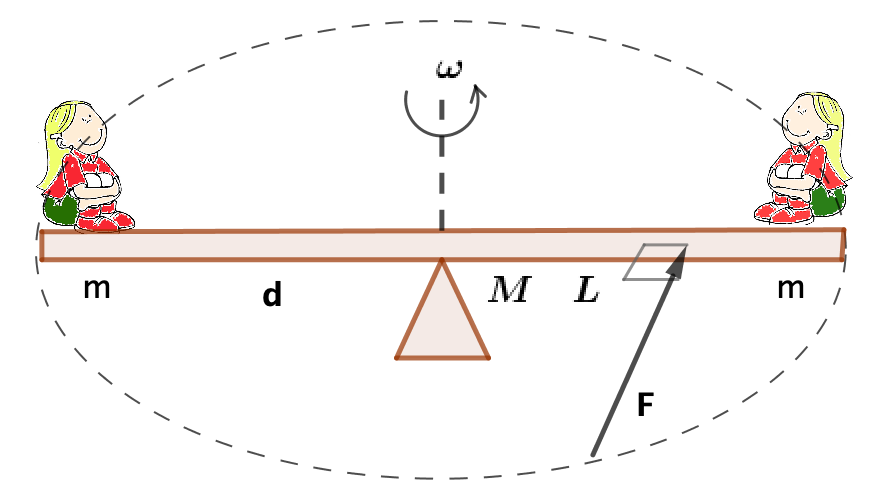
\includegraphics[width=.4\textwidth]{imagenes/imagenes16/T16IM20.png}
\end{figure}	
\end{multicols}

$Fr=I\alpha \to \alpha = \dfrac{Fr}{I}$, sustituyendo valores, $\ \alpha=1.33 \ \mathrm{rad\ s}^{-2}$

\begin{prob}
Un cilindro de $20 \ \mathrm{Kg}$ de masa y $0.25\ \mathrm{m}$ de radio está girando a $1200\ \mathrm{rpm}$ con respecto a un eje que pasa por su centro. ?`Cuál es la fuerza tangencial necesaria que habría que aplicar para que se detuviese en $1800$ revoluciones.
\end{prob}

$m=20 \ \mathrm{Kg}; \quad r=0.25\ \mathrm{m}; \quad \omega_0=1200\ \mathrm{rpm}=40\pi\  \mathrm{rad\ s}^{-1};$

$\theta=1800$ revoluciones = $3600\pi \ \mathrm{rad};\quad \omega=0 \  \mathrm{rad\ s}^{-1}$

$F=cte \to I\alpha=Fr,\quad \alpha=cte:\quad MCUA$, movimiento circular uniformemente acelerado, con aceleración angular negativa (de frenado, en realidad el movimineto es retardado)

Cuando se para: $\cancelto{0}{\omega}=\omega_0-\alpha t \to t=\dfrac{\omega_0} {\alpha}$

Ángulo barrido: $\theta=\cancelto{0}{\theta_0}+\omega_0 t - \dfrac 1 2 \alpha t^2$, sustituyendo ${t}$,

$\theta = \dfrac {\omega_0^2}{\alpha}-\dfrac 1 2 \cancel{\alpha}\dfrac{\omega_0^2}{\omega^{\cancel{2}}} \to \theta=\dfrac{\omega_0^2}{2\alpha} \ \Rightarrow \ \alpha=\dfrac{\omega_0^2}{2\theta}$

Por otro lado, $\displaystyle \dv {\vec L}{t}=\vec M^{(e)} \to I\alpha=Fr\sin 90^o=Fr \ \Rightarrow \ F=\dfrac{I\alpha}{r}$

$I=I{cilindro}=\dfrac 1 2 m r^2$, sustituyendo valores: $\ F=2.5 \times 10^4\ \mathrm{N}$

\rule{5cm}{.4pt}

\emph{Cálculo del momento de inercia de un cilindro homogéneo de masa $m$ y radio $r$ que gira entorno al eje longitudinal de simetría que pasa por el centro de masas}.

\begin{multicols}{2}
Cilindro homogéneo $M,\ H,\ R$

$\rho=\dfrac{M}{\pi R^2 H}$

$\dd m= \rho \dd V =\rho  \pi \left[ (r+\dd r)^2-r^2 \right] H=$

$=\rho \pi H \left[\cancel{r^2}+2r\dd r +\cancelto{0}{\dd^2 r}-\cancel{r^2} \right]$

$=2\pi \rho H r \dd r$

$\quad$

$I=\displaystyle \int_M r^2 \dd m$
\begin{figure}[H]
	\centering
	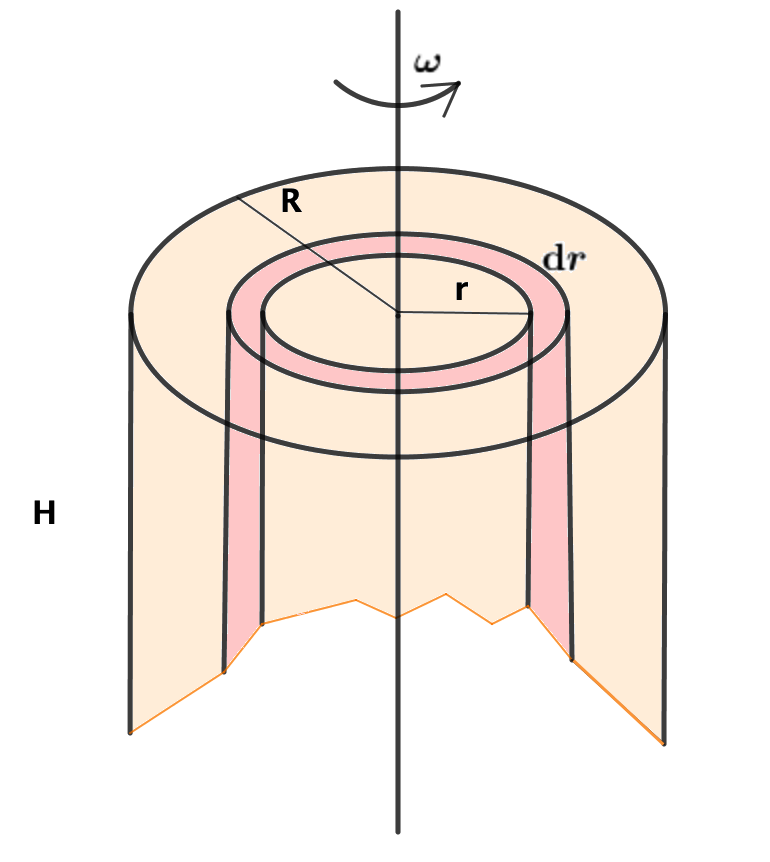
\includegraphics[width=.45\textwidth]{imagenes/imagenes16/T16IM22.png}
\end{figure}	
\end{multicols}

$\displaystyle I=2\pi \rho  H \int_0^R r^3 \dd r = 2 \pi \dfrac{M}{\pi R^2 H}H \dfrac{R^4}{4}=\dfrac 1 2 M R^2$

\begin{prob}
Demostrar que el momento de inercia	de un cuerpo rígido respecto a un eje que forma ángulos $\alpha,\ \beta,\ \gamma$ con los tres ejes principales es:
$\ \ I=I_1 \cos^2 \alpha + I_2 \cos^2 \beta + I_3 \cos^2 \gamma$
\end{prob}
\begin{multicols}{2}
$\quad$

$\mathcal E_c=\dfrac 1 2 I\omega = \dfrac 1 2 I_1 \omega_1^2+\dfrac 1 2 I_2 \omega_2^2+\dfrac 1 2 I_3 \omega_3^2$

$\quad$

$\begin{cases}
\quad \omega_1=\omega \cos \alpha \\
\quad\omega_2=\omega \cos \beta \\
\quad \omega_3=\omega \cos \gamma
\end{cases}$

\begin{figure}[H]
	\centering
	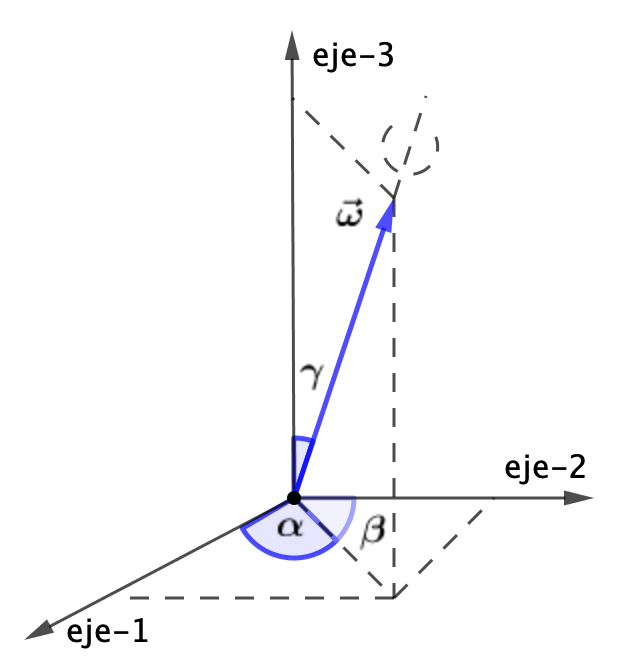
\includegraphics[width=.3\textwidth]{imagenes/imagenes16/T16IM23.png}
\end{figure}	
\end{multicols}
\vspace{-3mm} %***************************
$\mathcal E_c=\dfrac 1 2 \left( I_1 \cos^2 \alpha + I_2 \cos^2 \beta + I_3 \cos^2 \gamma \right)\omega^2$

$\text{Luego, } \quad   I=I_1 \cos^2 \alpha + I_2 \cos^2 \beta + I_3 \cos^2 \gamma \ ; \qquad \text{Teorema de Poinsot}$

\begin{prob}
Una esfera maciza rueda por dos planos inclinados distintos, di igual altura pero distinta inclinación.	?`Llegará la esfera al extremo inferior de los planos con la misma velocidad?, ?`empleará el mismo tiempo en llegar?
\end{prob}

\begin{multicols}{2}
$mgh=\frac 1 2 m V_{CM}^2+\frac 1 2 I \omega^2$

$v_{CM}=\omega R;\quad I=\frac 2 5 mR^2$

Luego $\ v=\sqrt{\frac {10}{7}gh}=cte$
\begin{figure}[H]
	\centering
	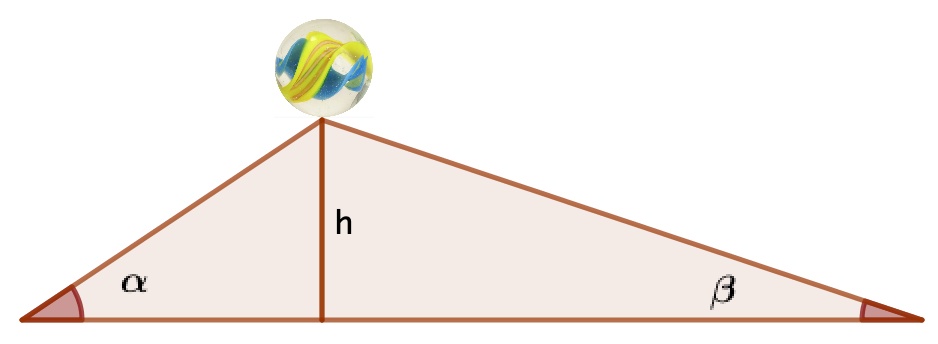
\includegraphics[width=.4\textwidth]{imagenes/imagenes16/T16IM24.png}
\end{figure}	
\end{multicols}
La esfera llega al final del plano con la misma velocidad, independientemente del ángulo $\theta$ de inclinación.

$v_{CM}=\displaystyle \dv{s}{t}; \quad h=s \sin \theta \to \dd x= \sqrt{\frac {10}{7}g \sin \theta \ s }\ \dd t \to \int_0^s \frac{\dd s}{\sqrt{s}}=\int_0^{t_\theta} \sqrt{\frac {10}{7}g\sin \theta}\dd t$

$\displaystyle 2\sqrt{x}= \sqrt{\frac {10}{7}g\sin \theta} \ t_\theta \to x=\frac {h}{\sin \theta}=\frac 5{14} g \sin \theta \ t^2_\theta \to h=\frac 5{14} g \sin^2 \theta \ t^2_\theta =cte$

Por lo que, $\sin^2 \theta \ t_\theta^2=cte \to \sin \theta \ t_{\theta}=cte$ y tendremos que

$t_\alpha \sin \alpha = t_\beta \sin \beta \ \Rightarrow \ \text{ si } \theta \uparrow \text{ entonces } t_\theta \downarrow\ $, la esfera cae antes (menor tiempo en caer) en el plano con mayor inclinación (ángulo mayor).


\rule{5cm}{0.3pt}
\vspace{1cm}
\begin{figure}[H]
	\centering
	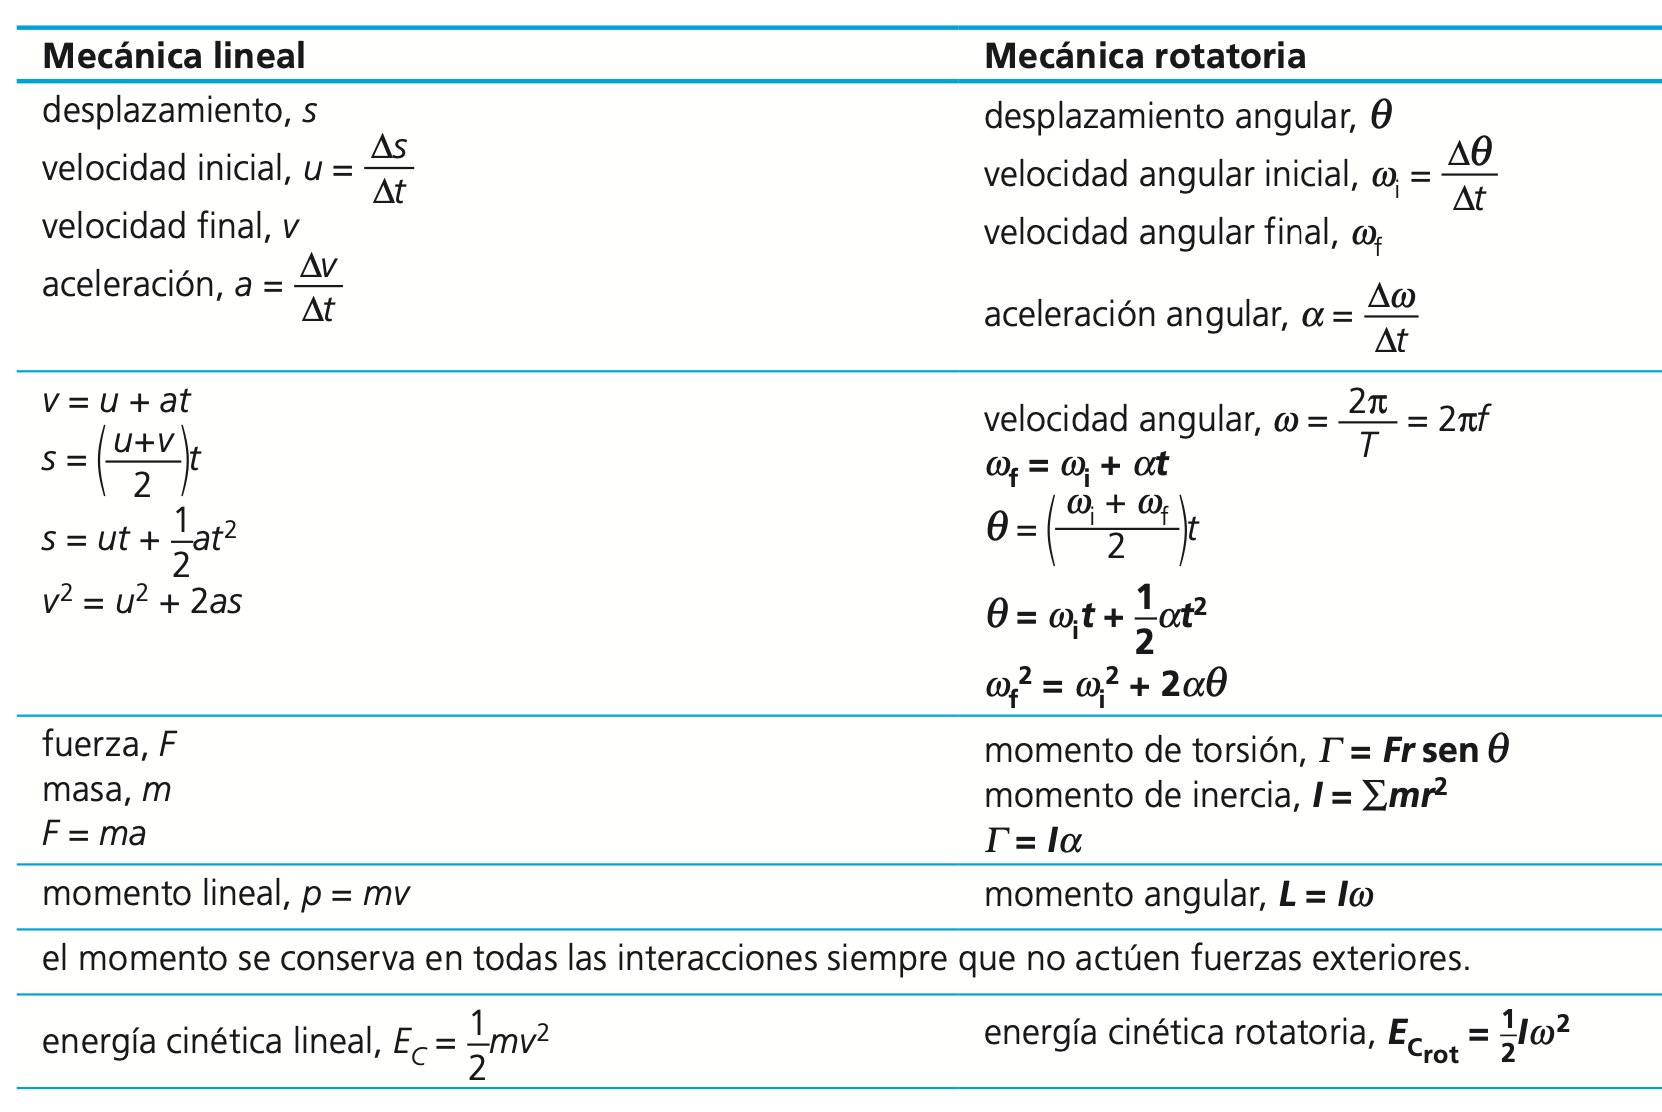
\includegraphics[width=1\textwidth]{imagenes/imagenes16/T16IM25.png}
\end{figure}



\newpage %******************************************************

\begin{myblock}{Momento de inercia y conservación del momento angular}

\vspace{2mm} \small{Si ningún momento externo actúa sobre un sistema en rotación, la cantidad de movimiento angular de ese sistema permanecerá constante.} 

\vspace{2mm} \small{Esto significa que, si no hay un momento externo, el producto de la inercia por la velocidad angular en un momento será igual que en cualquier otro momento $L=I\omega=cte$.}


\begin{figure}[H]
	\centering
	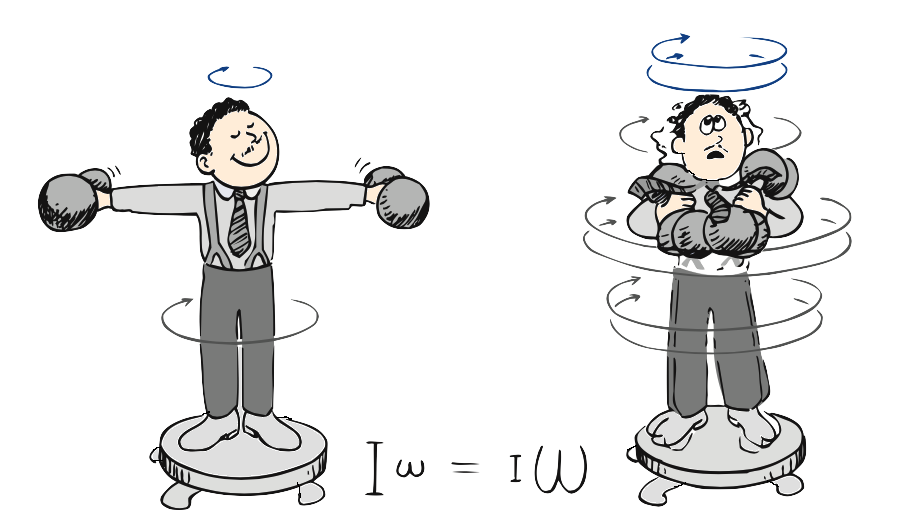
\includegraphics[width=.9\textwidth]{imagenes/imagenes16/T16IM07.png}
\end{figure}


\vspace{2mm} \small{Un ejemplo interesante que ilustra la conservación del momento angular se ve en la figura adjunta. El hombre está de pie sobre una mesa giratoria sin fricción, con las pesas extendidas. Su inercia $I$, con ayuda de las pesas extendidas, es relativamente grande en esa posición. Cuando gira con lentitud, su momento angular es el producto de su inercia por la velocidad de rotación, $\omega$. Cuando junta las pesas con su cuerpo, la inercia de su cuerpo y de las pesas se reduce en forma considerable. ?`Cuál es el resultado? !`Aumenta su rapidez de rotación! Este ejemplo lo aprecia mejor la persona que gira, que siente cambios de rapidez de rotación que le parecen misteriosos. ¡Pero es física en acción! Este procedimiento lo usan los patinadores artísticos que comienzan a girar con los brazos, y quizá una pierna, extendidos, para después juntar los brazos y la pierna, y así obtener una mayor rapidez de rotación. Siempre que un cuerpo que gira se contrae, aumenta su rapidez de rotación}\normalsize{.} 
	
\end{myblock}


